%===================================================================================
% Chapter: Dataset
%===================================================================================
\chapter{Análisis del conjunto de datos}\label{chapter:dataset}
% \addcontentsline{toc}{chapter}{Análisis del conjunto de datos}
%===================================================================================

En el proceso de entrenamiento y prueba de los algoritmos de aprendizaje de máquina, el conjunto de datos utilizado es de gran importancia, pero escoger uno lo suficientemente bueno no es tarea fácil. El conjunto KDDCup99 fue elaborado por el MIT Lincoln Lab patrocinado por DARPA en un escenario simulado donde realizaban ataques a la base de las fuerzas aéreas, lo cual tuvo una duración de 9 semanas \cite{mchugh2000testing}. Los datos fueron analizados y separados según el tipo de ataque o tráfico no malicioso de la red. Es uno de los conjuntos públicos disponibles que contiene ataques actuales y más utilizados para la construcción de IDS, lo que facilita la comparación de diferentes trabajos.

\section{Descripción del conjunto de datos}\label{section:dataset_description}
El conjunto de datos KDDCup99 posee aproximadamente 5 millones de datos los que se dividen en 5 clases:

\begin{itemize}
    \item Normal: tráfico común que navega por la red como puede ser el acceso a un sitio web o el envío de archivos no maliciosos.
    \item Negación de Servicios (DoS): esto es un ataque que ocupa gran parte del poder de cómputo o la memoria haciendo así que otras peticiones no puedan ser atendidas.
    \item Probing: un atacante escanea la red para ganar información que pueda explotar en el momento de infiltrarse en esta.
    \item Ataque remoto a un equipo local (R2L): el atacante envía paquetes a la red con el objetivo de explotar alguna vulnerabilidad disponible y ganar acceso local.
    \item User to Root (U2R): el atacante accede a la red desde una cuenta de usuario común y explota las vulnerabilidades existentes para ganar acceso como administrador en el sistema.
\end{itemize}

De igual forma, cada paquete contiene 41 características que pueden ser continuas o discretas. Estas están divididas en 4 categorías:

\begin{itemize}
    \item Características básicas que están derivadas de los encabezados de los paquetes sin inspeccionar los datos transmitidos.
    \item Características de contenido para los cuales se utiliza el conocimiento del dominio para evaluar la carga útil de los paquetes TCP originales.
    \item Características basadas en el tiempo de tráfico.
    \item Características basadas en el tráfico del host.
\end{itemize}

Este conjunto de datos tiene algunos problemas como el contenido de datos redundantes causando que los algoritmos de aprendizaje tengan una inclinación por los datos más frecuentes, el número de entradas para elaborar un conjunto de test puede variar en cada trabajo dado que el conjunto de datos no está separado, entre otros. Para eliminar algunos de estos errores se elaboró el conjunto NSL-KDD con un total de 1.1 millones de datos. A pesar de los esfuerzos, este aún sufre de algunos problemas tratados por McHugh \cite{mchugh2000testing} y no es una representación perfecta del contenido real en las redes. Por la falta de conjuntos de datos públicos, este puede ser un buen medidor para ayudar a las diferentes investigaciones y poderlas comparar entre sí. 

En adición, cada dato contiene un nivel de dificultad. Para lograr este objetivo se entrenaron 7 algoritmos diferentes, cada uno 3 veces, y a cada dato que aceptaron se le incrementó en uno el valor de dificultad, siendo 21 el valor máximo representando el nivel de dificultad más bajo. El conjunto de datos en su totalidad consta de 8 archivos:

\begin{itemize}
    \item KDDTrain+.arff : el conjunto de entrenamiento completo con los datos clasificados en normal y anómalos.
    \item KDDTrain+.txt : el conjunto de entrenamiento completo con los datos clasificados según el tipo de ataque y el nivel de dificultad.
    \item KDDTrain+\_20Percent.arff : subconjunto de 20\% del archivo KDDTrain+.arff.
    \item KDDTrain+\_20Percent.txt : subconjunto de 20\% del archivo KDDTrain+.txt.
    \item KDDTest+.arff : conjunto de prueba completo con los datos clasificados en normal y anómalos. Posee datos diferentes y algunas clasificaciones de ataques nuevas con respecto al conjunto de entrenamiento.
    \item KDDTest+.txt : conjunto de prueba completo con los datos clasificados según el tipo de ataque y el nivel de dificultad. Posee datos diferentes y algunas clasificaciones de ataques nuevas con respecto al conjunto de entrenamiento.
    \item KDDTest-21.arff : subconjunto de KDDTest+.arff que no contiene los datos con dificultad 21 de 21.
    \item KDDTest-21.txt : subconjunto de KDDTest+.txt que no contiene los datos con dificultad 21 de 21.
\end{itemize}

\begin{table}[h]
    \begin{center}
        \caption{Cantidad de datos en cada subconjunto.}

        \label{tab:len_datasets}
        \begin{tabular}{c|c|c|c} % <-- Alignments: 1st column left, 2nd middle and 3rd right, with vertical lines in between
        \textbf{KDDTrain+} & \textbf{KDDTrain+\_20Percent} & \textbf{KDDTest+} & \textbf{KDDTest-21}\\
        \hline
        125973 & 25192 & 22544 & 11850\\
        \end{tabular}
    \end{center}
\end{table}

\section{Pre procesamiento de los datos}
Con el objetivo de optimizar el proceso de aprendizaje y los resultados obtenidos por los algoritmos es necesario realizar un pre procesamiento de los datos. Este consiste en la transformación y normalización de los datos dado que existen campos con valores reales y otros con dominio definido. Para los campos con valores binarios reales no es necesario realizar ninguna transformación \cite{patro2015normalization}.

Los campos con valores reales tienen como valor mínimo el 0 por lo que el proceso de normalización consiste en buscar el valor máximo de cada campo y dividir todos los valores por este. En el caso de los campos con dominio definido, como lo es protocol\_type que sus valores pertenecen al dominio \{'tcp', 'udp', 'icmp'\}, se le asigna un valor entero a cada posible valor, igual al su indice en la lista de posibles valores, y luego se dividen entre el máximo valor que es igual a la cantidad de valores posibles menos uno. Después de estos procesos todos los campos de los datos poseen valores entre 0 y 1.

\section{Selección de características}
Los mecanismos de selección de características ayudan a identificar y remover las no esenciales, irrelevantes y redundantes de los datos que no influyen en la precisión de los resultados. La selección de características es el proceso que indica cual es la mejor representación de los datos para resolver un problema determinado. Si este proceso no se aplica, puede tener un efecto negativo en la precisión de las respuestas de los modelos de predicción \cite{tuv2009feature}.

Uno de los métodos más utilizados para lograr este objetivo es el de bosques aleatorios. Este clasificador ha brindado buenos resultados para el problema en cuestión. Es un algoritmo basado en árboles que se utiliza en problemas de clasificación y ayuda a obtener la importancia de las características en cada uno. Se puso a prueba en el conjunto NSL-KDD y de un total de 41 características se descartaron 11 que aportaban poca información sobre la clasificación de los datos, quedando así 30 para el entrenamiento de los algoritmos clasificadores.

\section{Clasificación}
\begin{table}[b]
    \begin{center}
        \caption{Asociación de los tipos de ataques a sus categorías.}
        
        \label{tab:class}
        \begin{tabular}{l|l} % <-- Alignments: 1st column left, 2nd middle and 3rd right, with vertical lines in between
        \textbf{Categorías} & \textbf{Tipos de ataques}\\
        \hline
        DoS & back, land, neptune, pod, smurf, teardrop, mailbomb,\\ 
        & apache2, processtable, udpstorm\\
        Probe & ipsweep, nmap, portsweep, satan, mscan, saint\\
        R2L & ftp write, guess passwd, imap, multihop, phf, spy,\\
        & warezclient, warezmaster, sendmail, named,\\
        & snmpgetattack, snmpguess, xlock, xsnoop, worm\\
        U2R & buffer overflow, loadmodule, perl, rootkit, httptunnel,\\
        & ps, sqlattack, xterm\\
        \end{tabular}
    \end{center}
\end{table}

La clasificación es el proceso de predicción de los datos luego de que el algoritmo seleccionado sea entrenado. En el caso de este conjunto de datos específico las entradas poseen varias clases. Como se mencionó con anterioridad este trabajo se centra solo en la clasificación binaria, debido a que en la práctica es más importante la detección de un ataque que su clasificación. A pesar de esto, el conocimiento del tipo del ataque puede ayudar a una prevención mas adecuada. Las diferentes clases presentes en NSL-KDD se muestran en la tabla \ref{tab:class}.

A pesar de que este conjunto de datos tiene grandes virtudes, no es perfecto. Algo que lo perjudica son las cantidades de datos en cada una de las categorías de ataques. Como muestra la tabla \ref{tab:atk_counts} hay tipos de ataques que poseen una mayor cantidad de entradas lo cual puede causar una inclinación en los algoritmos de aprendizaje de máquina.

\begin{table}[h]
    \begin{center}
        \caption{Distribución de los datos en los subconjuntos de entrenamiento y prueba.}
        
        \label{tab:atk_counts}
        \begin{tabular}{c|c|c|c|c|c|c} % <-- Alignments: 1st column left, 2nd middle and 3rd right, with vertical lines in between
        \textbf{} & \textbf{Normal} & \textbf{DoS} & \textbf{Probe} & \textbf{U2R} & \textbf{R2L} & \textbf{Total}\\
        \hline
        \textbf{Train} & 67343 & 45927 & 11656 & 52 & 995 & 125973\\
        \textbf{Test} & 9711 & 7458 & 2421 & 200 & 2754 & 22544\\
        \end{tabular}
    \end{center}
\end{table}

\section{Conjunto de datos original}
Para las primeras pruebas se utilizó el conjunto de datos en su forma original. Los procesos de entrenamiento y validación se llevaron a cabo particionando el subconjunto KDDTrain en un 80\% y 20\% para cada una de las tareas respectivamente. En la fase de prueba se le aplicaron a los modelos ambos conjuntos, KDDTest+ y KDDTest-21, debido a la diferencia de dificultad entre estos se puede tener una mejor estimación de los resultados que se obtendrán en condiciones reales. Esta diferencia se debe a la forma en que se elaboraron, KDDTest+ en su mayoría posee datos de ataques mostrando una mayor relación de casos anómalos contra normales que KDDTrain. Por otra parte, KDDTest-21 es un subconjunto de KDDTest+ que solo posee datos con dificultad menor o igual a 20, excluyendo así los mas fáciles. Para una mejor noción de las diferencias de dificultades en la figura \ref{fig:diff_distribution} se muestra la distribución de los datos en los conjuntos KDDTrain y KDDTest según su dificultad.

% TODO: ponerle los números de las cantidades a las gráficas
\begin{figure}
    \centering
    \subfigure{\label{fig:kddtrain_distribution}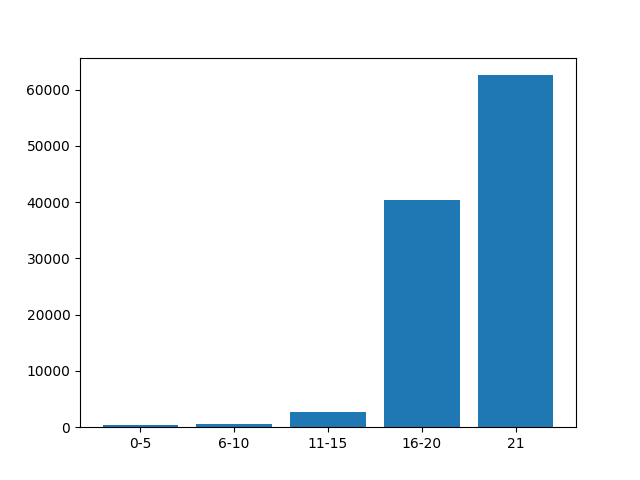
\includegraphics[width=.45\linewidth]{Images/distribution_train.png}}
    \subfigure{\label{fig:kddtest_distribution}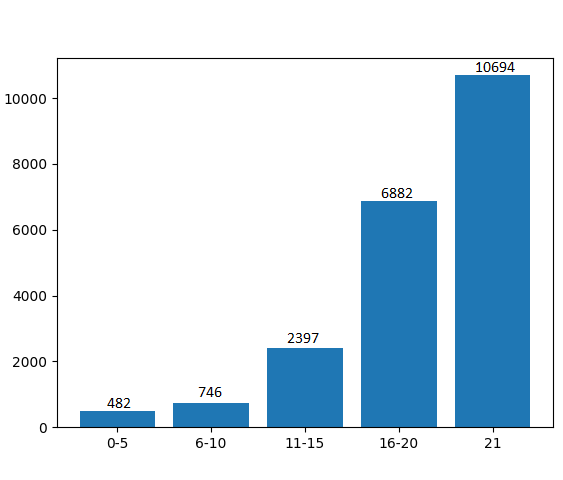
\includegraphics[width=.45\linewidth]{Images/distribution_test.png}}

    \caption{Distribución de datos por dificultad en los conjuntos KDDTrain y KDDTest respectivamente.}
    \label{fig:diff_distribution}
\end{figure}

Para una mayor precisión en los resultados se utilizó el método k-fold \cite{10.5555/3203489}. Este consiste en dividir el conjunto de entrenamiento en $k$ particiones, creando $k$ modelos idénticos y entrenando el i-esimo con las $k - 1$ restantes mientras que se evalúan con la i-esima partición. Luego de obtener los $k$ resultados se promedian. El valor de $k$ escogido fue de 5 (usualmente se trabaja con 5 o 4) con 100 epochs y un tamaño de batch de 64. Al comienzo de este proceso se desordenaron los datos del conjunto de entrenamiento de modo aleatorio.

\section{Conjunto de datos modificado}
A pesar de que loas pruebas y los resultados aquí obtenidos se desarrollan bajo un entorno de laboratorio, el producto final esta destinado al uso en redes reales. En esas condiciones, aunque el modelo debe comportarse correctamente ante datos nuevos que no observó en su fase de entrenamiento, a este se le van a mostrar la mayor variedad de datos para que posea un mejor conocimiento. Por estas razones se decidió unificar el conjunto KDDTrain y KDDTest en uno, desordenar los datos de modo aleatorio y luego volver a particionar este en un 80\% y 20\% para las fases de entrenamiento y prueba. Con el objetivo de obtener una mejor estimación del comportamiento de los modelos, este proceso se realizó 10 veces, luego se promediaron todos los resultados y esta fue la cifra que se tuvo en cuenta. Cabe destacar que en cada una de las iteraciones se unificó el conjunto de datos, se desordenó y se volvió a particionar.